\hypertarget{the-odd-couple}{%
\section{The Odd Couple}\label{the-odd-couple}}

\begin{figure}[!ht]
  \begin{adjustwidth}{-\oddsidemargin-1in}{-\rightmargin}
    \centering
    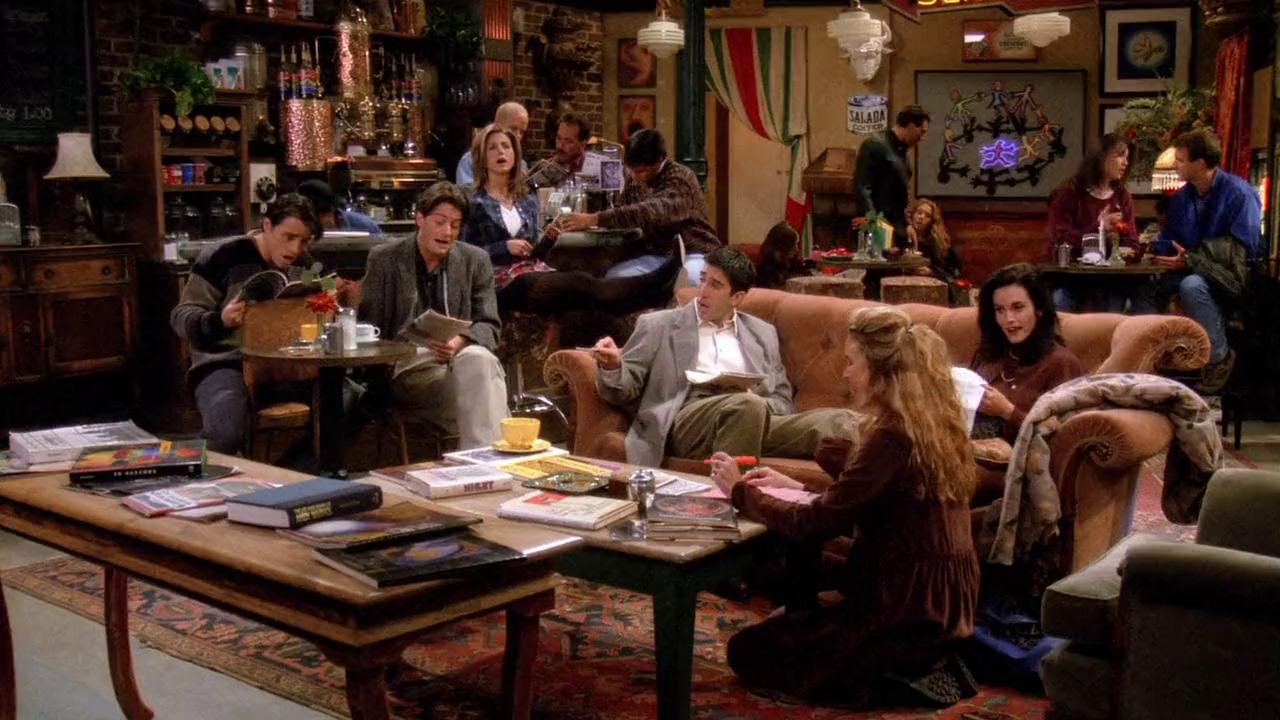
\includegraphics[trim={0 6cm 0 2cm,}, clip, width=\paperwidth]{./S01/img/12/the-odd-couple.png}
    % \caption{The Odd Couple\label{fig:the-odd-couple}}
  \end{adjustwidth}
\end{figure}

A música cantada logo no início do episódio é o tema de abertura da
série \emph{The Odd Couple} (1970-1975), que conta a história de dois
amigos tentando dividir um apartamento, mas cada um tem uma maneira de
viver muito diferente e isso gera muitos conflitos.

\textbf{Matthew Perry} ainda estrelou uma releitura da série em 2015
junto com \emph{Thomas Lennon}, com a mesma premissa.

\begin{figure}
  \centering
  \begin{tikzpicture}
    \node [inner sep=0pt] at (0,0) {
      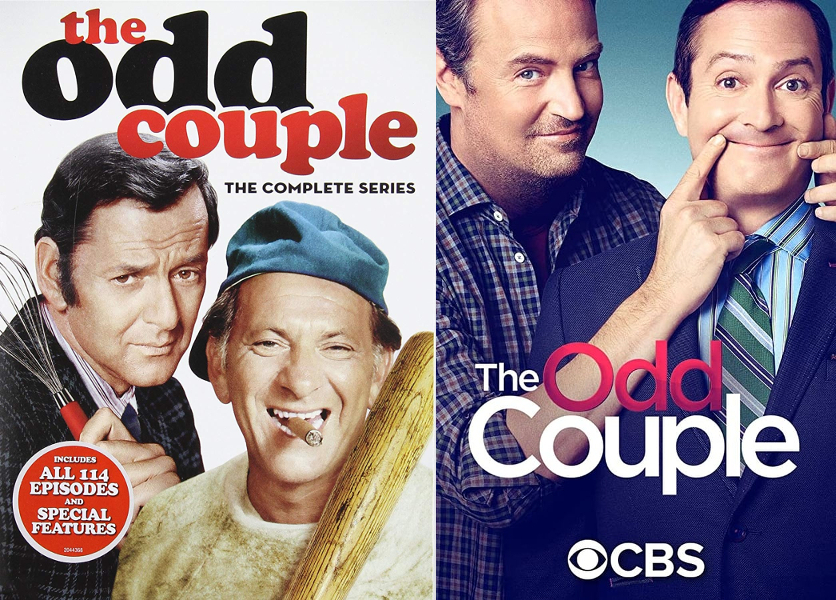
\includegraphics[width=0.7\textwidth,keepaspectratio]{./S01/img/12/the-odd-couple-poster.jpg}
    };
    \draw [white, rounded corners=\ClipSep, line width=\ClipSep]
    (current bounding box.north west) --
    (current bounding box.north east) --
    (current bounding box.south east) --
    (current bounding box.south west) -- cycle
    ;
    \end{tikzpicture}
    \caption{The Odd Couple - Poster\label{fig:the-odd-couple-poster}}
\end{figure}

\hypertarget{referuxeancias}{%
\subsection{Referências}\label{referuxeancias}}

\begin{itemize}
\tightlist
\item
  \sloppy Fandom Wiki. \url{https://friends.fandom.com/wiki/The_One_With_The_Dozen_Lasagnas}
\item
  \sloppy TMDB. \url{https://www.themoviedb.org/tv/1809-the-odd-couple}
\item
  \sloppy IMDB. \url{https://www.imdb.com/title/tt0065329/?ref_=tt_sims_tt}
\item
  \sloppy Tema de abertura (1970) - YouTube. \url{https://www.youtube.com/watch?v=kDrfHj3j398}
\item
  \sloppy Tema de abertura (2015) - YouTube. \url{https://www.youtube.com/watch?v=mrsj4yd_c3I}
\end{itemize}

\hypertarget{i-dream-of-jeannie}{%
\section{I Dream of Jeannie}\label{i-dream-of-jeannie}}

\begin{figure}[!ht]
  \begin{adjustwidth}{-\oddsidemargin-1in}{-\rightmargin}
    \centering
    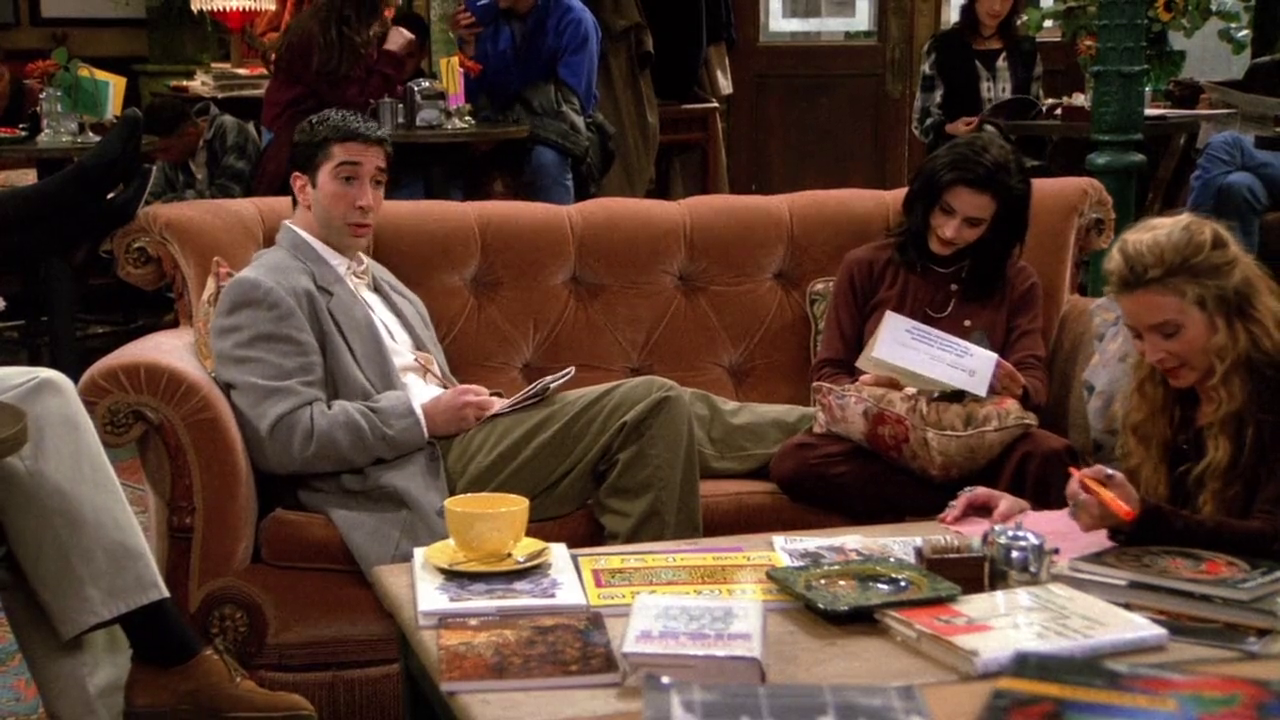
\includegraphics[trim={0 6cm 0 2cm,}, clip, width=\paperwidth]{./S01/img/12/i-dream-of-jeannie.png}
    % \caption{I Dream of Jeannie\label{fig:i-dream-of-jeannie}}
  \end{adjustwidth}
\end{figure}

Logo após a bem sucedida vocalização de \emph{The Odd Couple}, Ross
tenta emendar o tema de \emph{I Dream of Jeannie} (1965-1970),
\emph{sitcom} americana que conta a história de \emph{Tony Nelson}, um
astronauta que liberta um gênio da garrafa, \emph{Jeannie}.

\begin{figure}
  \centering
  \begin{tikzpicture}
    \node [inner sep=0pt] at (0,0) {
      
\includegraphics[width=0.4\textwidth,keepaspectratio]{./S01/img/12/i-dream-of-jeannie-poster.jpg}
    };
    \draw [white, rounded corners=\ClipSep, line width=\ClipSep]
    (current bounding box.north west) --
    (current bounding box.north east) --
    (current bounding box.south east) --
    (current bounding box.south west) -- cycle
    ;
    \end{tikzpicture}
    \caption{I Dream of Jeannie - Poster\label{fig:i-dream-of-jeannie-poster}}
\end{figure}

\begin{tcolorbox}[enhanced,center upper,
    drop fuzzy shadow southeast, boxrule=0.3pt,
    lower separated=false,
    colframe=black!30!dialogoBorder,colback=white]
\begin{minipage}[c]{0.16\linewidth}
  \raisebox{\dimexpr-\height+\ht\strutbox\relax}{
    \centering 
\includegraphics[width=1.4cm]{./assets/img/chandler.png}
  }
   & \centering \scriptsize{Chandler}
\end{minipage}
\hfill
\begin{minipage}[c]{0.8\linewidth}
  \textbf{- No, no, we're done. We're done, man.}\\
  - Não, já chega, já chega cara.
\end{minipage}
\end{tcolorbox}

O tema é referenciado novamente em
\textbf{\textcolor{primarycolor}{S08E20 - Aquele com o chá de bebê}},
quando Joey está praticando para seu \emph{game show Bamboozled}, onde
ele pergunta a Ross:

\begin{quote}
\emph{Audio question: Name this television theme song\ldots{}}
\end{quote}

\hypertarget{referuxeancias-1}{%
\subsection{Referências}\label{referuxeancias-1}}

\begin{itemize}
\tightlist
\item
  \sloppy Fandom Wiki. \url{https://friends.fandom.com/wiki/The_One_With_The_Dozen_Lasagnas}
\item
  \sloppy TMDB. \url{https://www.themoviedb.org/tv/1660-i-dream-of-jeannie}
\item
  \sloppy Bamboozled - Fandom Wiki. \url{https://friends.fandom.com/wiki/Bamboozled}
\end{itemize}

\hypertarget{huey-lewis}{%
\section{Huey Lewis}\label{huey-lewis}}

\begin{figure}[!ht]
  \begin{adjustwidth}{-\oddsidemargin-1in}{-\rightmargin}
    \centering
    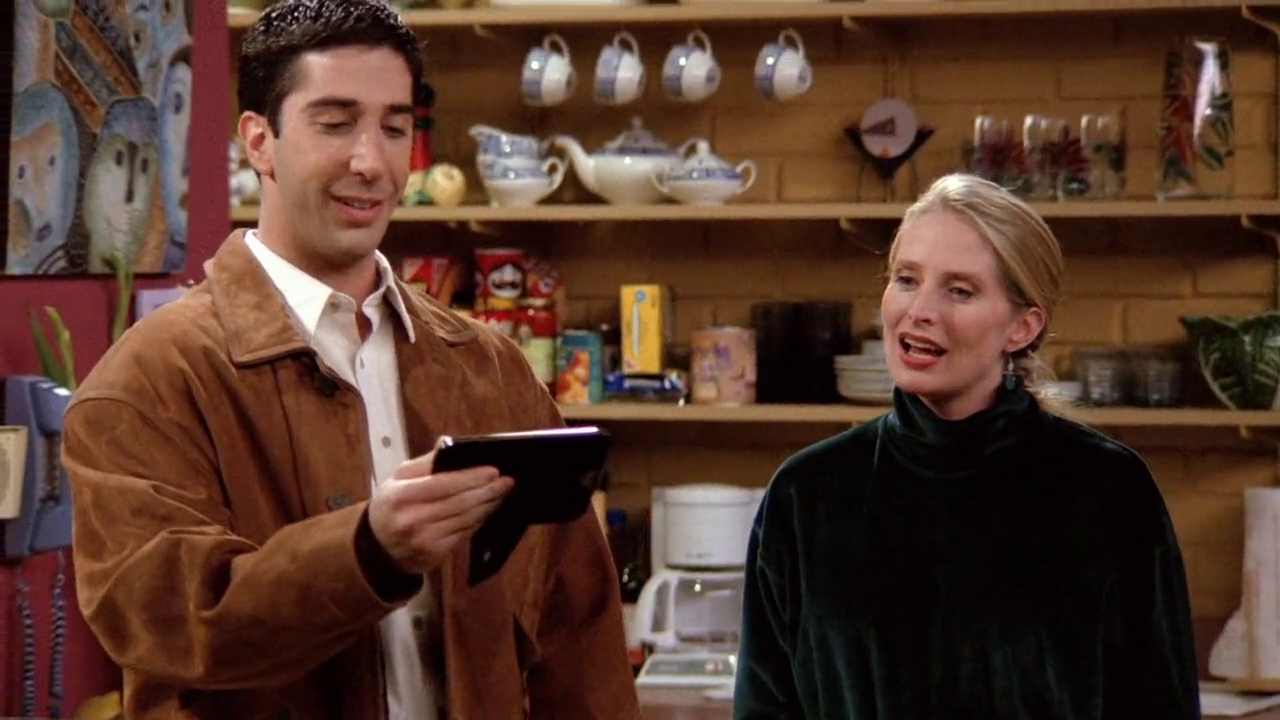
\includegraphics[trim={0 7cm 0 0cm,}, clip, width=\paperwidth]{./S01/img/12/huey-lewis.png}
    % \caption{Huey Lewis\label{fig:huey-lewis}}
  \end{adjustwidth}
\end{figure}

\begin{tcolorbox}[enhanced,center upper,
    drop fuzzy shadow southeast, boxrule=0.3pt,
    lower separated=false,
    colframe=black!30!dialogoBorder,colback=white]
\begin{minipage}[c]{0.16\linewidth}
  \raisebox{\dimexpr-\height+\ht\strutbox\relax}{
    \centering 
\includegraphics[width=1.4cm]{./assets/img/ross.png}
  }
   & \centering \scriptsize{Ross}
\end{minipage}
\hfill
\begin{minipage}[c]{0.8\linewidth}
  \textbf{- Hey. When did you and Susan meet Huey Lewis?}\\
  - Quando vocês conheceram Huey Lewis?
\end{minipage}

\medskip
\begin{minipage}[c]{0.16\linewidth}
  \raisebox{\dimexpr-\height+\ht\strutbox\relax}{
    \centering 
\includegraphics[width=1.4cm]{./assets/img/carol.png}
  }
   & \centering \scriptsize{Carol}
\end{minipage}
\hfill
\begin{minipage}[c]{0.8\linewidth}
  \textbf{- Uh, that's our friend Tanya.}\\
  - Essa é nossa amiga Tanya.
\end{minipage}

\medskip
\begin{minipage}[c]{0.16\linewidth}
  \raisebox{\dimexpr-\height+\ht\strutbox\relax}{
    \centering 
\includegraphics[width=1.4cm]{./assets/img/ross.png}
  }
   & \centering \scriptsize{Ross}
\end{minipage}
\hfill
\begin{minipage}[c]{0.8\linewidth}
  \textbf{- Of course it's your friend Tanya.}\\
  - Claro que é sua amiga Tanya.
\end{minipage}
\end{tcolorbox}

\emph{Hugh Anthony Cregg III} ou simplesmente \emph{Huey Lewis} (1950-)
é um cantor, compositor e ator americano. É o vacalista principal e toca
gaita na banda \emph{Huey Lewis and the News} (1980).

\begin{figure}
  \centering
  \begin{tikzpicture}
    \node [inner sep=0pt] at (0,0) {
      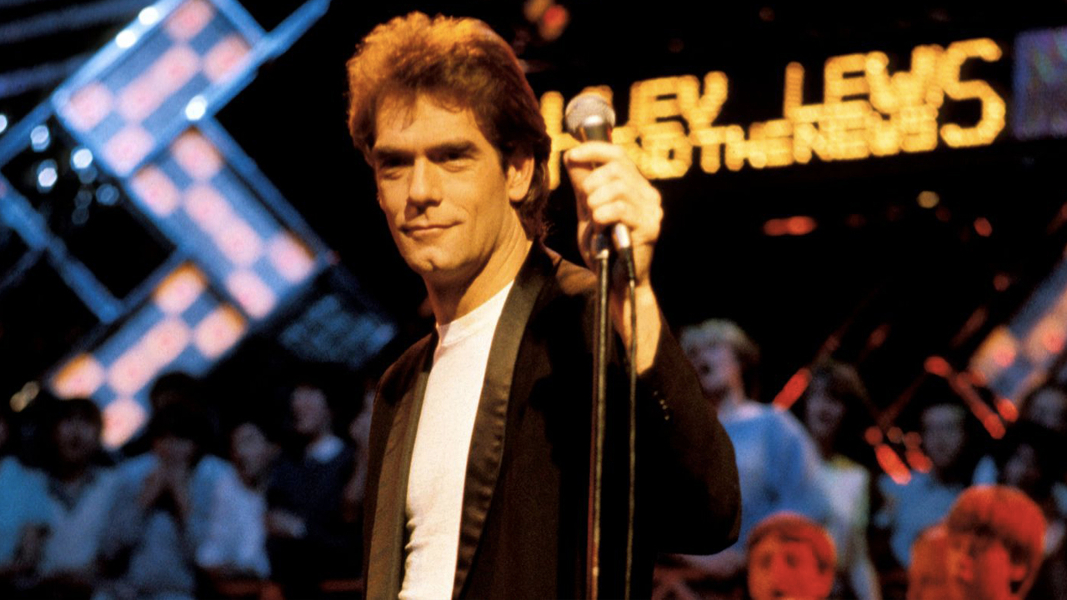
\includegraphics[width=0.8\textwidth,keepaspectratio]{./S01/img/12/huey-lewis-and-the-news.jpeg}
    };
    \draw [white, rounded corners=\ClipSep, line width=\ClipSep]
    (current bounding box.north west) --
    (current bounding box.north east) --
    (current bounding box.south east) --
    (current bounding box.south west) -- cycle
    ;
    \end{tikzpicture}
    \caption{Huey Lewis and the News\label{fig:huey-lewis-and-the-news}}
\end{figure}

\hypertarget{referuxeancias-2}{%
\subsection{Referências}\label{referuxeancias-2}}

\begin{itemize}
\tightlist
\item
  \sloppy Twitter. \url{https://twitter.com/HueyLewisNews}
\item
  \sloppy Wikipédia. \url{https://en.wikipedia.org/wiki/Huey_Lewis}
\item
  \sloppy Site oficial da banda. \url{http://www.hueylewisandthenews.com/}
\end{itemize}

\hypertarget{hibachi}{%
\section{Hibachi}\label{hibachi}}

\begin{figure}[!ht]
  \begin{adjustwidth}{-\oddsidemargin-1in}{-\rightmargin}
    \centering
    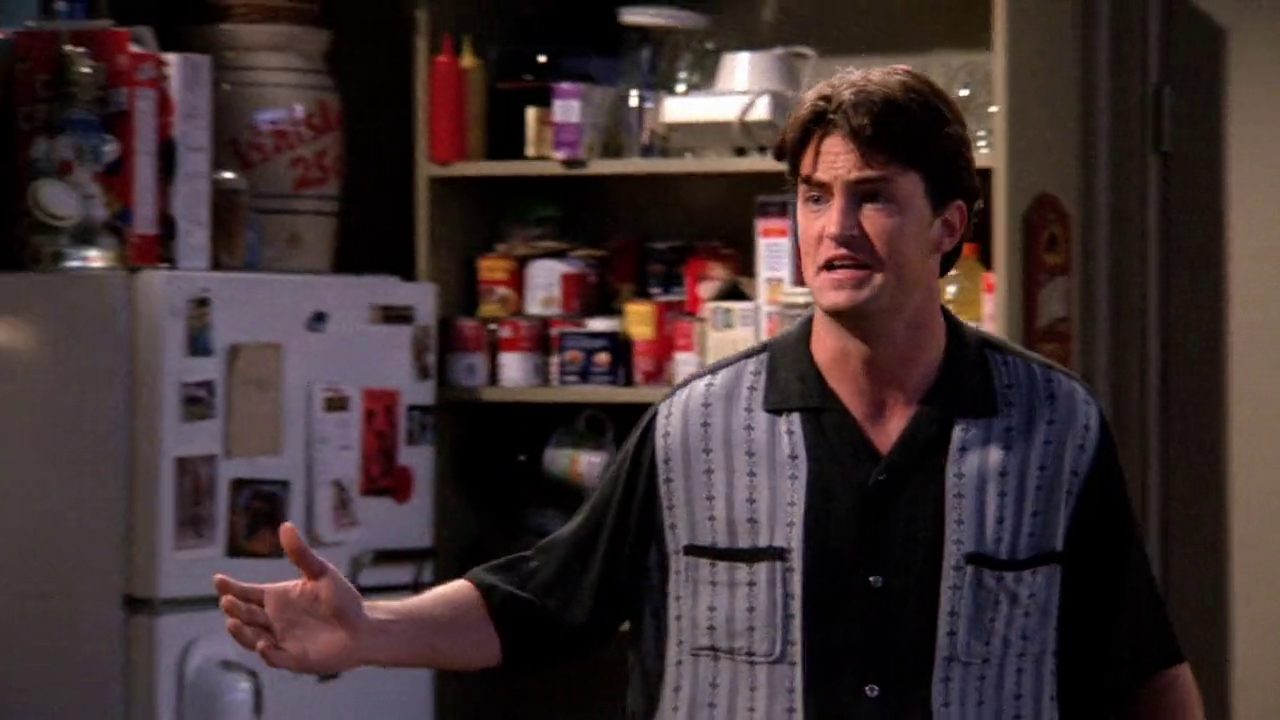
\includegraphics[trim={0 7cm 0 1cm,}, clip, width=\paperwidth]{./S01/img/12/hibachi.png}
    % \caption{Hibachi\label{fig:hibachi}}
  \end{adjustwidth}
\end{figure}

\begin{tcolorbox}[enhanced,center upper,
    drop fuzzy shadow southeast, boxrule=0.3pt,
    lower separated=false,
    colframe=black!30!dialogoBorder,colback=white]
\begin{minipage}[c]{0.16\linewidth}
  \raisebox{\dimexpr-\height+\ht\strutbox\relax}{
    \centering 
\includegraphics[width=1.4cm]{./assets/img/chandler.png}
  }
   & \centering \scriptsize{Chandler}
\end{minipage}
\hfill
\begin{minipage}[c]{0.8\linewidth}
  \textbf{- We bought a hibachi together, and then he ran off and got married... and things got pretty ugly.}\\
  - Compramos um hibachi juntos, ele se casou...  e as coisas ficaram feias.
\end{minipage}
\end{tcolorbox}

Chandler menciona que comprou um \emph{hibachi} com \emph{Kip}, mas
depois que ele casou acabou levando o aparelho, que nada mais é que uma
espécie de chapa para preparar comida. No episódio
\textbf{\textcolor{primarycolor}{S01E14 - Aquele com os Corações Doces}},
podemos ver um \emph{hibachi} no restaurante japonês onde Ross e Kristen
se encontram com Carol e Susan.

\begin{figure}
  \centering
  \begin{tikzpicture}
    \node [inner sep=0pt] at (0,0) {
      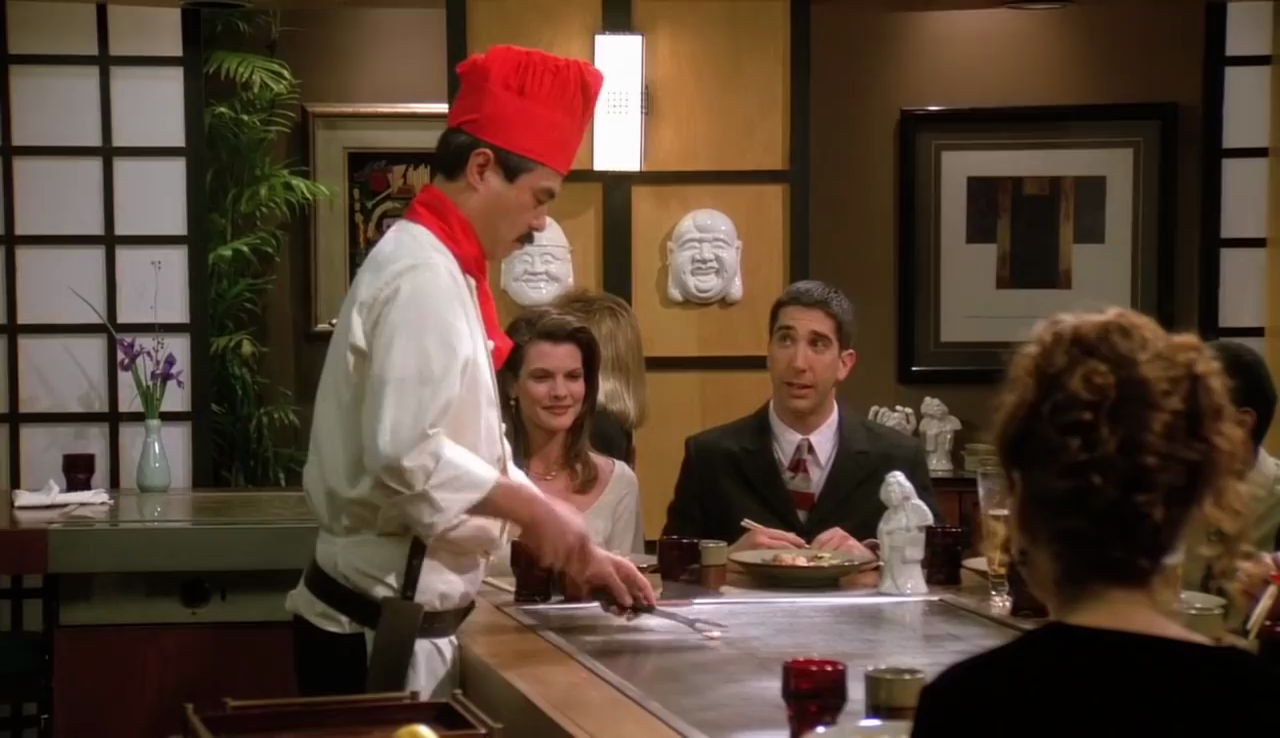
\includegraphics[width=0.8\textwidth,keepaspectratio]{./S01/img/12/hibachi-ross-carol.png}
    };
    \draw [white, rounded corners=\ClipSep, line width=\ClipSep]
    (current bounding box.north west) --
    (current bounding box.north east) --
    (current bounding box.south east) --
    (current bounding box.south west) -- cycle
    ;
    \end{tikzpicture}
    \caption{S01E14 - Hibachi\label{fig:s01-e14-hibachi}}
\end{figure}

\hypertarget{referuxeancias-3}{%
\subsection{Referências}\label{referuxeancias-3}}

\begin{itemize}
\tightlist
\item
  \sloppy Shinto Restaurants (Inglês). \url{https://shintorestaurants.com/what-is-hibachi/}
\end{itemize}
